\chapter{KDE桌面环境的一些配置}
KDE桌面环境中通过系统设置以及应用程序的设置可以极大的进行自定义,从而提高工作效率。
\section{系统设置}
\subsection{字体设置}
正式文档排版一般都需要宋体、黑体、仿宋、楷体这些字体,从\href{http://pan.baidu.com/s/1mgiHWmO}{百度云}下载好后点击或者用zypper即可安装。开源字体如Ubuntu字体(\soft{ubuntu-fonts})和文泉驿微米黑(\soft{wqy-microhei-fonts})等则可以直接在源中找到甚至默认已经安装好了。

对于非root程序,在\menu{应用程序外观}\me\menu{字体设置}中,你可以调节各种字体字号,当然对于屏幕显示字体最好选择无衬线字体,如Droid Sans Fallback、各种黑体。图\ref{myfont}就是我的相关字体设置。
\begin{figure}[htbp!]
 \centering
 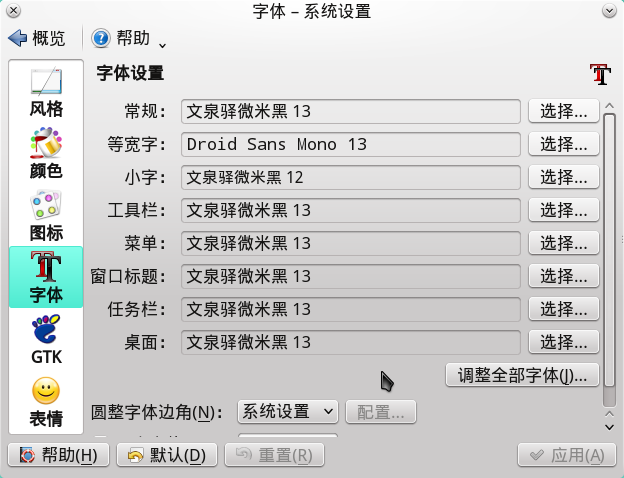
\includegraphics[width=\textwidth]{./pic/fontsettings.png}
 \caption{我的字体设置}\label{myfont}
\end{figure}

对于root程序,比如YaST的字体设置,你需要在终端中以root权限运行系统设置(\command{systemsettings})再单独设置。再次强调,在openSUSE中为了能够以root运行相关图形程序,需要使用\command{kdesu}来代替\command{sudo}。

\subsection{桌面效果设置}
在\menu{桌面效果}\me\menu{全部效果}中可以启用各种桌面特效,如模糊效果、半透明效果、桌面立方效果和屏幕反色等功能。

注意,过多的效果可能导致运行缓慢,如果您觉得您的电脑运行缓慢请关闭某些特效。
\subsection{开机自启动管理}
在\menu{开机和关机}\me\menu{自动启动}中可以管理你的启动项。

在\menu{开机和关机}\me\menu{会话管理}中可以关掉或者打开开机时恢复上一次会话。如果你选择打开,那么上次注销或关机时没有关闭的程序在下次登录后会被启动。但这样显然就拖慢了开机速度。
\subsection{快捷键的设置}
在\menu{快捷方式和手势}\me\menu{自定义快捷键}中你可以为程序或命令设置相应的快捷键,这样你就可以抛弃桌面图标了——所有常用的程序通过快捷键启动,非常用的程序用启动器或Krunner启动。

在\menu{快捷方式和手势}\me\menu{标准键盘快捷键}中你可以设置KDE程序内通用的快捷键,如查找、上一页、第一页、保存、退出等。

在\menu{快捷方式和手势}\me\menu{全局键盘快捷键}中你可以设置各种KDE组件的快捷键。例如在KWin中设置好切换桌面与窗口的快捷键你就可以切换起来如鱼得水。例如我的切换桌面到上下左右采用的是类似于VIM的Ctrl+Alt+k/j/h/l。这一切你都可以自由定制。
\subsection{外观设置}
在工作空间外观或者应用程序外观中可以调节相应的外观。

例如在\menu{工作空间外观}\me\menu{窗口装饰}\me\menu{配置按钮}中你可以调整标题栏按钮的位置。我自己采取左关右小的设置可以使关闭和最小化全屏应用程序极为方便,而最大化及恢复只需双击标题栏即可。
\begin{figure}[htbp!]
 \centering
 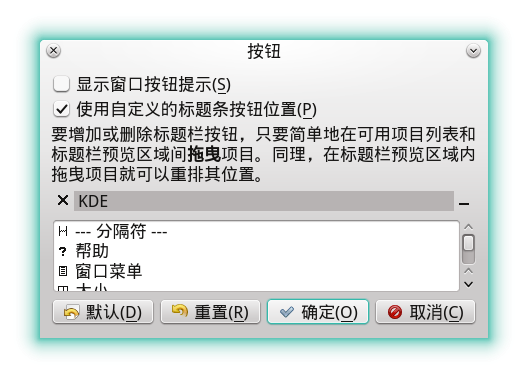
\includegraphics{./pic/botton.png}
 \caption{配置按钮}\label{botton}
\end{figure}

另外很多主题都可以在kde-look上下载或者通过获得新装饰获得。
\subsection{活动、桌面与Plasma桌面挂件}
活动是比桌面大的一个层次,每个活动可以有自己的桌面。而桌面挂件就是一些放在面板或者桌面上的小工具。

桌面空白处右键菜单中选择活动就可以管理活动。另外你可以通过Meta+Tab切换活动。
\begin{figure}[htbp!]
\centering
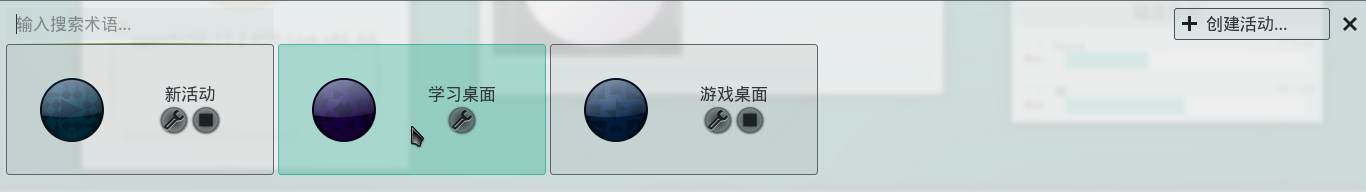
\includegraphics[width=\textwidth]{./pic/activity.png} 
\caption{活动管理}\label{activity}
\end{figure}

按Ctrl+F$i(i=1234\ldots)$可以切换到对应桌面。对应虚拟桌面的一些选项你可以在\menu{工作空间行为}\me\menu{虚拟桌面}中进行设置。对于某个活动中的一组桌面有很多类型可选。在桌面空白处右键菜单中选择桌面设置后你可以选择切换各种布局类型(例如桌面图标就和Windows如出一辙)以及切换壁纸等。
\begin{figure}[htbp!]
\centering
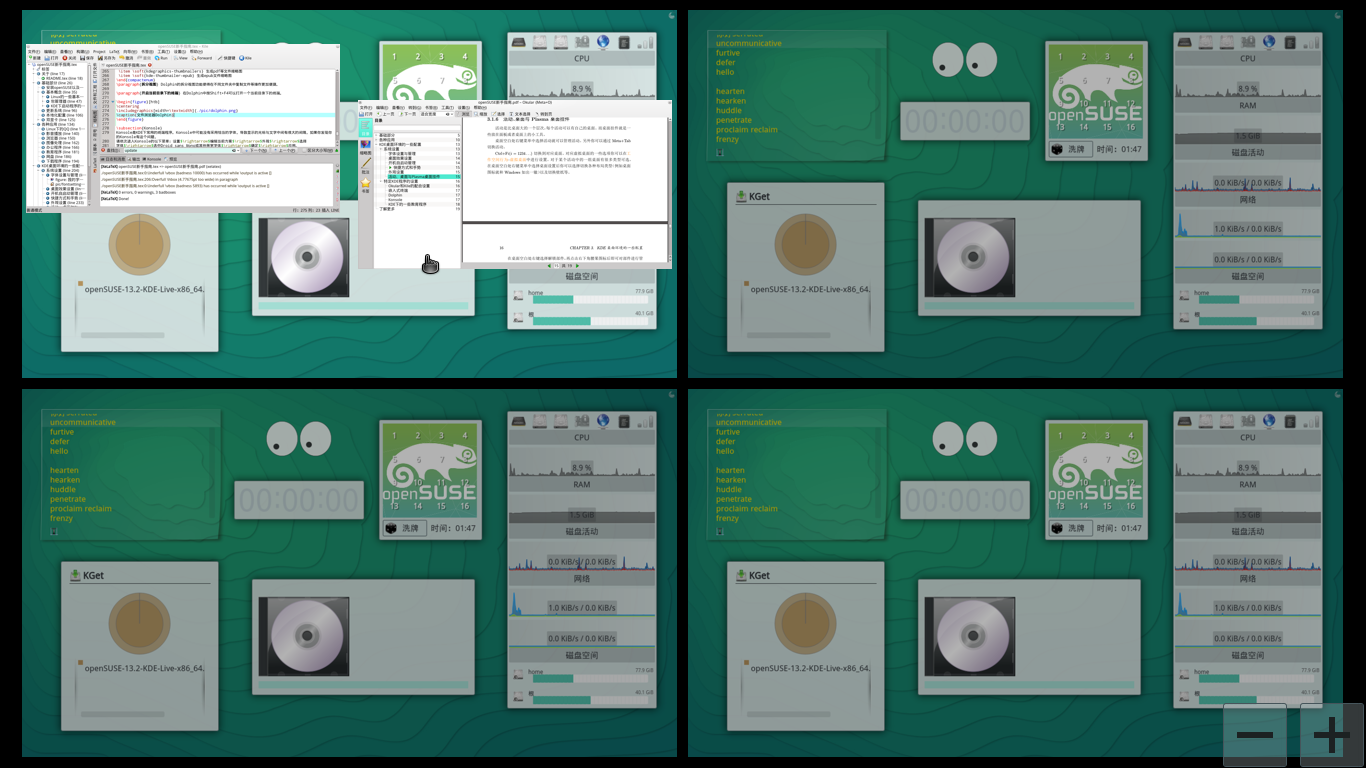
\includegraphics[width=\textwidth]{./pic/virtualdesk.png} 
\caption{多个虚拟桌面}\label{multidesk}
\end{figure}

在桌面空白处右键选择解锁部件,再点击右下角腰果图标后即可对部件进行管理。例如安装好\soft{redshift}及\soft{plasmoid-redshift}挂件后使你能够方便的调节屏幕色温,保护视力(你也可以让它隐藏在系统托盘里)。
添加部件时你既可以双击添加到面板,也可以托拽到桌面去。
\begin{figure}[htbp!]
\centering
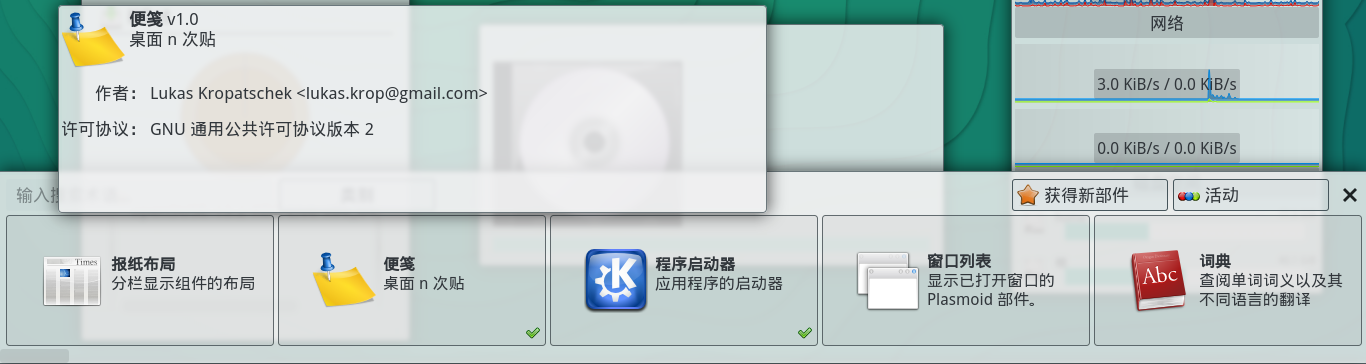
\includegraphics[width=\textwidth]{./pic/plasma.png} 
\caption{添加桌面小挂件}\label{plasma}
\end{figure}

\section{特定KDE程序的设置}
基本所有的KDE程序都可以进行详细的配置,比如工具栏等。在工具栏中添加好常用的图标可以让你每次用的时候都少点几次鼠标。
\subsection{Okular和Kile的配合设置}
编写\LaTeX文档时常用Okular作为pdf阅读器,Kile等作为编辑器。\href{http://zpj.blog.ustc.edu.cn/?p=338}{这里}介绍了Kile与Okular的正反向搜索设置。

\subsection{嵌入式终端}
在Kile中点击右下侧的消息栏上的\menu{Konsole}即出现嵌入式终端。

Dolphin中按F4即可启用/退出嵌入式终端。

Kate中可以启用终端工具视图插件,之后设置好相应快捷键或者启用侧边栏即可方便的启用嵌入式终端。
\subsection{Dolphin}
Dolphin是KDE下默认的文件浏览器,按Ctrl+M可以显示菜单栏,不然就会华而不实。
\begin{figure}[htbp!]
\centering
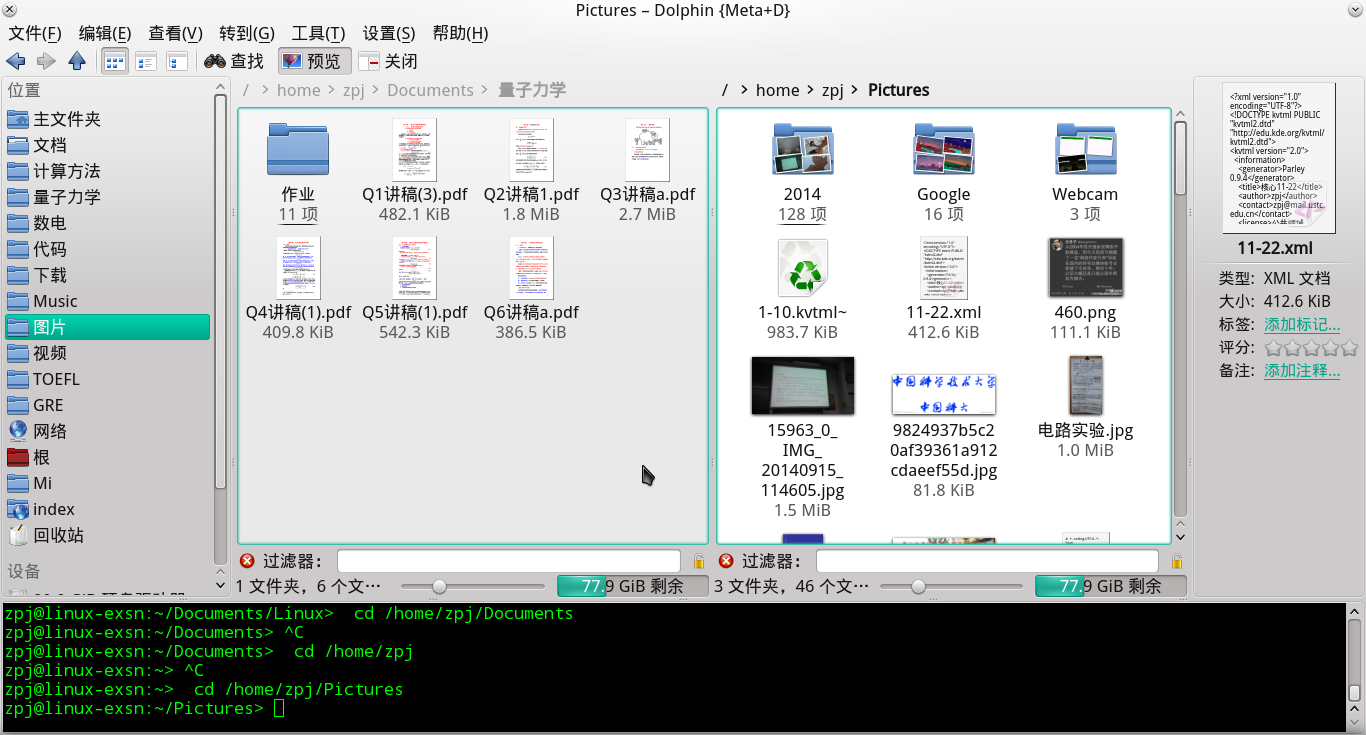
\includegraphics[width=\textwidth]{./pic/dolphin.png} 
\caption{Dolphin的拆分视图以及嵌入式终端}
\end{figure}

\paragraph{缩略图} Dolphin可以开启缩略图功能,在配置菜单的常规中的预览中选中相应条目即可。如果没有你想要的条目比如pdf,那么你可以用thumbnail为关键字,搜索源中相应的软件包并安装即可。比如:
\begin{compactenum}
 \item \soft{kffmpegthumbnailer} 生成视频文件缩略图
 \item \soft{kdegraphics-thumbnailers} 生成pdf等文件缩略图
\end{compactenum}
\paragraph{拆分视图} Dolphin的拆分视图功能使得在不同文件夹中复制文件等操作更加便捷。

\paragraph{开启当前目录下的终端} 在Dolphin中按Shift+F4可以打开一个当前目录下的终端。


\subsection{Konsole}
Konsole是KDE下常用的终端程序。Konsole中可能没有采用恰当的字体,导致显示的光标与文字中间有很大的间隔,如果你发现你的Konsole有这个问题,
请依次进入Konsole的以下菜单:\menu{设置}\me\menu{编辑当前方案}\me\menu{外观}\me\menu{选择
字体}\me选中Droid sans Mono或其他等宽字体\me确定并应用。

在Konsole的编辑配置方案中你可以选择不同的颜色方案等,适用于不同环境。你甚至可以在管理配置方案中为每个方案单独设置一个快捷键。
\subsection{KDE下的一些其他程序}
\paragraph{Parley} 一个背单词的程序,可以参考我对它的\href{http://zpj.blog.ustc.edu.cn/?p=294}{介绍}。

\paragraph{KTouch} 一个练习打字的程序。

\paragraph{Klipper} 剪贴板工具,一般位于系统托盘中,可以记录剪贴板历史和生成剪贴板内容的二维码。

\paragraph{Akregator} 一个本地RSS客户端。

\paragraph{KSnapshot} 截图工具,默认快捷键是PrtSc。另外,最好在\menu{桌面效果}\me\menu{全部效果}中启用\menu{屏幕截图}以使其功能与桌面特效更好地配合。